\documentclass[12pt]{article}
\usepackage[spanish]{babel}
\usepackage{natbib}
\usepackage{url}
\usepackage[utf8x]{inputenc}
\usepackage{amsmath}
\usepackage{hyperref}
\usepackage[style=listgroup,acronym,toc,hyperfirst,xindy]{glossaries}
\makeglossaries
\usepackage[xindy]{imakeidx}
\makeindex
\usepackage{wrapfig}
\usepackage{graphicx}
\graphicspath{{images/}}
\usepackage{parskip}
\usepackage{fancyhdr}
\usepackage{vmargin}
\setmarginsrb{3 cm}{2.5 cm}{3 cm}{2.5 cm}{1 cm}{1.5 cm}{1 cm}{1.5 cm}

\setglossarystyle{long}

\newacronymstyle{ex-footnote}%
{%
	\GlsUseAcrEntryDispStyle{footnote}%
}%
{%
	\GlsUseAcrStyleDefs{footnote}%
	\renewcommand*{\genacrfullformat}[2]{%
		\firstacronymfont{\glsentryshort{##1}}##2%
		\expandafter\footnote\expandafter{\expandafter\glsentrylong\expandafter{##1}}%
	}%
	\renewcommand*{\Genacrfullformat}[2]{%
		\firstacronymfont{\Glsentryshort{##1}}##2%
		\expandafter\footnote\expandafter{\expandafter\glsentrylong\expandafter{##1}}%
	}%
	\renewcommand*{\genplacrfullformat}[2]{%
		\firstacronymfont{\glsentryshortpl{##1}}##2%
		\expandafter\footnote\expandafter{\expandafter\glsentrylongpl\expandafter{##1}}%
	}%
	\renewcommand*{\Genplacrfullformat}[2]{%
		\firstacronymfont{\Glsentryshortpl{##1}}##2%
		\expandafter\footnote\expandafter{\expandafter\glsentrylongpl\expandafter{##1}}%
	}%
}

\setacronymstyle{ex-footnote}



%Glossary
\newglossaryentry{vhfg}
{
	name=VFH,
	description={Banda del espectro electromagnético que ocupa el rango de frecuencias de 30 MHz a 300 MHz}
}
\newglossaryentry{uhfg}
{
	name=UFH,
	description={Banda del espectro electromagnético que ocupa el rango de frecuencias de 300 MHz a 3 GHz}
}

% Acronym list
\newacronym{oscar}{OSCAR}{Orbiting Satellite Carrying Amateur Radio}
\newacronym{satnogs}{SatNOGS}{Satellite Networked Operation Ground Stations}


\title{Diseño de una antena helicoidal \\para radioenlace satelital en UHF}								% Title
\author{Alberto Mur López \\ Diego Cajal Orleans}								% Author
\date{\today}											% Date

\makeatletter
\let\thetitle\@title
\let\theauthor\@author
\let\thedate\@date
\makeatother

\pagestyle{fancy}
\fancyhf{}
\rhead{\theauthor}
\lhead{\thetitle}
\cfoot{\thepage}

\begin{document}

%%%%%%%%%%%%%%%%%%%%%%%%%%%%%%%%%%%%%%%%%%%%%%%%%%%%%%%%%%%%%%%%%%%%%%%%%%%%%%%%%%%%%%%%%

\begin{titlepage}
	\centering
    \vspace*{0.5 cm}
    
\includegraphics[scale = 0.75]{eina.png}\\[1.0 cm]	% University Logo
%    \textsc{\LARGE University of Cape Town}\\[2.0 cm]	% University Name
	\textsc{\Large 30340}\\[0.5 cm]				% Course Code
	\textsc{\large equipos y sistemas de transmisión}\\[0.5 cm]				% Course Name
	\rule{\linewidth}{0.2 mm} \\[0.4 cm]
	\setlength{\baselineskip}{2\baselineskip}
	{ \huge \bfseries \thetitle}\\
	\rule{\linewidth}{0.2 mm} \\[1.5 cm]
	
	\begin{minipage}{0.4\textwidth}
		\begin{flushleft} \large
			\emph{Autores:}\\
			\theauthor
			\end{flushleft}
			\end{minipage}~
			\begin{minipage}{0.4\textwidth}
			\begin{flushright} \large
			\emph{Nia:} \\
			565825 \\
			658212
												% Your Student Number
		\end{flushright}
	\end{minipage}\\[2 cm]
	
	{\large \thedate}\\[2 cm]
 
	\vfill
	
\end{titlepage}

%%%%%%%%%%%%%%%%%%%%%%%%%%%%%%%%%%%%%%%%%%%%%%%%%%%%%%%%%%%%%%%%%%%%%%%%%%%%%%%%%%%%%%%%%

\tableofcontents
\pagebreak

%%%%%%%%%%%%%%%%%%%%%%%%%%%%%%%%%%%%%%%%%%%%%%%%%%%%%%%%%%%%%%%%%%%%%%%%%%%%%%%%%%%%%%%%%

\section{Introducción}
Desde su descubrimiento casi accidental, la antena helicoidal operando en modo axial es una de las antenas más usadas para UHF y comunicaciones de microondas. El término axial hace referencia a la tendencia de la antena a radiar en la dirección de su extremo (axialmente), en lugar de lateralmente, cuando su radio es del orden de una longitud de onda.\\\\
El modo axial radia con polarización circular de forma predominante. En comunicaciones espaciales, así como en comunicaciones móviles terrestres, la orientación relativa entre la transmisión y recepción con polarización lineal no está garantizada, por lo que es necesario utilizar este tipo de polarización. Además, para aplicaciones espaciales, la rotación de Faraday a través de la ionosfera es, generalmente, impredecible (el plasma magnetizado en la ionosfera rota la dirección de la polarización lineal, pero no tiene efecto sobre la polarización circular). Por estas razones, es común que las antenas polarizadas linealmente experimenten desvanecimientos profundos, haciendo las comunicaciones poco fiables.\\\\
En el presente documento se va a detallar el diseño de una antena helicoidal para realizar un enlace satelital. Su frecuencia central estará en torno a los 435 MHz (UHF) y trabajará en modo axial. Los satélites objetivo son satélites de radio amateur, designados habitualmente como \gls{oscar}, que operan en la banda de UHF y VHF. La motivación de este proyecto viene de la necesidad de construir un seguidor de satélites basado en el proyecto \gls{satnogs}.\\\\
Para la realización de este trabajo se emplearán las herramientas Matlab y 4nec2.

\newpage
\section{Fundamentos teóricos}
Es interesante ver la estructura geométrica de una antena helicoidal no como un tipo básico de antena, sino como una particularización de un caso general. Una hélice de un diámetro fijo colapsa en una espira si el espacio entre sus vueltas se aproxima a cero. Como caso opuesto, si se fija el espacio entre sus vueltas, colapsa en un conductor rectilíneo cuando se reduce su diámetro.

\begin{figure}[h]
	\centering
	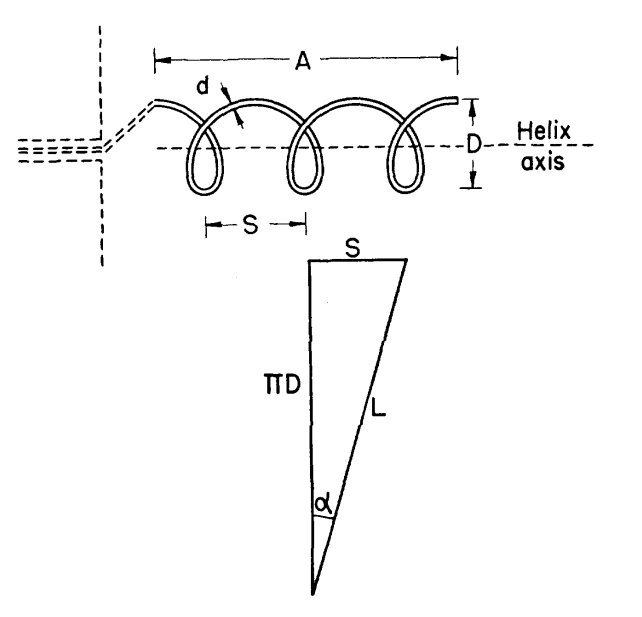
\includegraphics[width=0.40\textwidth]{parametros.png}
	\caption{Relación de dimensiones de la hélice}
	\label{fig:param}
\end{figure}

Normalmente, cuando se hable de dimensiones de la antena se hará en función de longitudes de onda (dimensiones eléctricas).

\subsection{Modos de transmisión y radiación de las hélices}
El campo electromagnético alrededor de la hélice puede ser tratado desde dos puntos de vista: como campo guiado y como campo radiado. Desde el primer punto de vista se asume que la onda electromagnética se propaga sin atenuación a lo largo de una hélice infinita, del mismo modo que lo haría por una linea de transmisión infinita. Esta propagación se puede describir por su \textit{modo de transmisión}. Por otro lado, el punto de vista del campo radiado se describe mediante el diagrama de radiación de la antena. Aunque son posibles una infinita variedad de diagramas, dos tipos son de particular interés dependiendo de la dirección del máximo de propagación: el modo de radiación normal y el modo de radiación axial.\\\\
El modo de transmisión de menor orden en un conductor helicoidal es el modo $T_{0}$. En él las regiones de carga positiva y negativa están separadas por varias vueltas. Es el modo de transmisión predominante cuando la longitud de una vuelta es mucho menor que la longitud de onda ($L<<\lambda$), común en inductores de baja frecuencia. Como las regiones adyacentes de carga están separadas por una distancia axial apreciable, aparece una componente axial de campo eléctrico. Esta componente interactúa con la onda viajera a lo largo de la hélice, dando lugar a campos radiados en la dirección normal. El caso más interesante asociado a este modo de transmisión se da cuando la longitud total de la antena es mucho menor que la longitud de onda ($nL<<\lambda$, siendo $n$ el número total de vueltas). En estas condiciones se puede asumir que las corrientes en la hélice tienen una magnitud y fase uniformes a lo largo de la estructura. De forma teórica, esta condición puede ser aproximada a una pequeña hélice cargada en su extremo en la que se produce una onda estacionaria. La impedancia de la antena se vuelve dependiente de la frecuencia y la eficiencia de radiación es pequeña. Esta combinación de antena pequeña con el modo de transmisión $T_{0}$ da lugar a antenas helicoidales con modo de radiación normal. La antena a diseñar requiere un modo de radiación axial, que no puede ser conseguido con dicho modo de transmisión.\\

\begin{figure}[h]
	\centering
	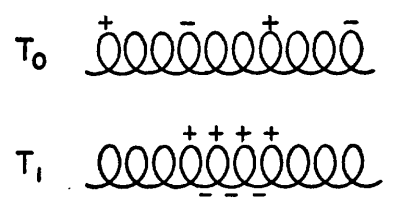
\includegraphics[width=0.3\textwidth]{modos.png}
	\caption{Distribución de las cargas para diferentes modos de transmisión}
	\label{fig:modes}
\end{figure}

El modo de transmisión de primer orden, designado como $T_{1}$, tiene las regiones de cargas positivas y negativas separadas aproximadamente por media vuelta de hélice, haciendo que queden diametralmente opuestas. Es el modo predominante cuando la longitud de una vuelta es del orden de una longitud de onda ($L\sim\lambda$). La radiación de este tipo de helices cuando $n>1$ tiene el máximo en la dirección de la hélice y está polarizada circularmente. Este tipo de radiación es el que se conoce como modo axial y es el que se quiere conseguir para la antena a diseñar. Una de las características más importantes de este modo de radiación es que se produce para un amplio rango de dimensiones de la hélice, haciendo que sea una de las antenas más fáciles de construir.\\\\
Los modos de radiación normal y axial son en realidad casos particulares de diagramas de radiación de antenas helicoidales. En el caso general, el máximo de radiación no estará ni en $\theta=0$ ni en $\theta=90º$, sino en un valor intermedio.

\subsection{Modo de radiación axial}
Las distribuciones de corriente de una antena helicoidal funcionando en modo axial pueden describirse como una onda viajera saliente más una onda viajera entrante de mucha menos magnitud. Cada onda está caracterizada por una región inicial de fuerte atenuación seguida de otra en la que la corriente es relativamente constante.\\

\begin{figure}[!h]
	\centering
	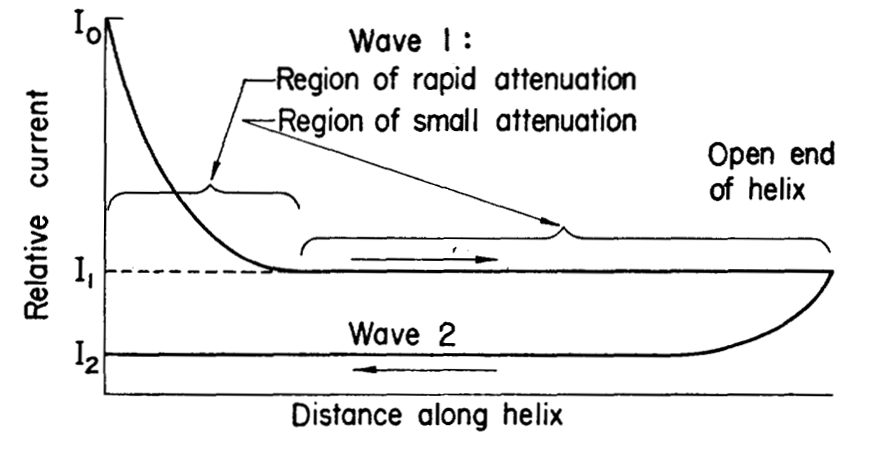
\includegraphics[width=0.6\textwidth]{ondas.png}
	\caption{Distribuciónes de corriente idealizadas}
	\label{fig:waves}
\end{figure}

La profunda atenuación de la onda reflejada (entrante) permite una distribución uniforme en la zona central en hélices largas. Ambas atenuaciones, tanto de la saliente como de la reflejada, explican la relativa estabilidad en impedancia de este tipo de antenas, ya que relativamente poca energía de la reflejada en el extremo llega a la entrada. Así, la SWR de corriente a la entrada es

\begin{equation*}
	SWR=\frac{I_{0}+I_{2}}{I_{0}-I_{2}}\approx 1
\end{equation*}

lo mismo que para una línea de transmisión cargada con su impedancia característica.\\\\
La velocidad de fase de la onda en la hélice es tal que hace que la componente del campo eléctrico en cada vuelta se sume aproximadamente en fase en la dirección del eje. La tendencia a que esto ocurra es lo suficientemente fuerte para que la velocidad de fase se ajuste por si misma para producir este resultado. Este ajuste natural es el que hace que el modo axial tenga su persistencia característica.\\\\
La velocidad de fase es aproximadamente igual a la velocidad de la luz en el vacío cuando la frecuencia es muy baja para el modo de radiación axial. Si se aumenta la frecuencia, aparece un rango frecuencial en el que la velocidad de fase es menor. En este rango es en el que radia en  dirección axial.

\subsection{Factor de agrupación}
Como aproximación, se asume que en modo axial se tiene una única onda viajera saliente en el conductor. El diagrama de la hélice es calculado como una agrupación de vueltas individuales, todas con el mismo diagrama de radiación. Cuando la antena es lo suficientemente larga ($nS$ grande), el factor de agrupación se vuelve dominante y determina casi por completo la forma del diagrama. Así, aunque las componentes de polarización vertical y horizontal de cada vuelta son muy diferentes, las componentes de la hélice completa son prácticamente iguales.\\\\
Para calcular el factor de agrupación, la hélice de $n$ vueltas se remplaza por $n$ fuentes puntuales isotrópicas.

\begin{equation}
	FA(\psi)=\frac{\sin\frac{n\psi}{2}}{\sin\frac{\psi}{2}}
\end{equation} 

La fase con la que la onda radiada por la \textit{fuente 1} llega a un punto arbitrario $P$ está adelantada a la fase de la onda proveniente de la \textit{fuente 2} por $2\pi S_{\lambda}\cos\theta$, pero retardada por $2\pi L_{\lambda}/p$, donde $p$ es el factor de velocidad de fase ($p=v/c$). Este retardo es proporcional al tiempo requerido para que la onda viaje a lo largo de una vuelta, de la fuente 2 a la 1. El valor del ángulo eléctrico $\psi$ es la diferencia.

\begin{equation}
	\psi=2\pi(S_{\lambda}\cos\theta-\frac{L_{\lambda}}{p})
\end{equation} 

Las ondas llegan a $P$ en fase cuando $\psi=-2\pi m$ y $\theta=0$, donde $m$ es un entero $(0,1,2,...)$. Se puede extraer la siguiente condición:

\begin{equation}
	\frac{L_{\lambda}}{p}=m+S_{\lambda}
\end{equation} 

La expresión (3) se relaciona de forma directa con los modos de transmisión comentados en la sección 2.1, ya que es una relación aproximada para que por el conductor existan los diferentes modos $T_{m}$. Así, para el modo $T_{1}$, que es el que produce radiación axial, tenemos:

\begin{equation}
	\frac{L_{\lambda}}{p}=1+S_{\lambda}\longrightarrow\frac{L}{p}=\lambda+S
\end{equation} 

Introduciendo la relación $L²=S²+(\pi D)²$, se obtiene una interrelación entre los parámetros de espaciado ($S$) y diámetro ($D$) para que la antena radie en modo axial.\\

\begin{figure}[!h]
	\centering
	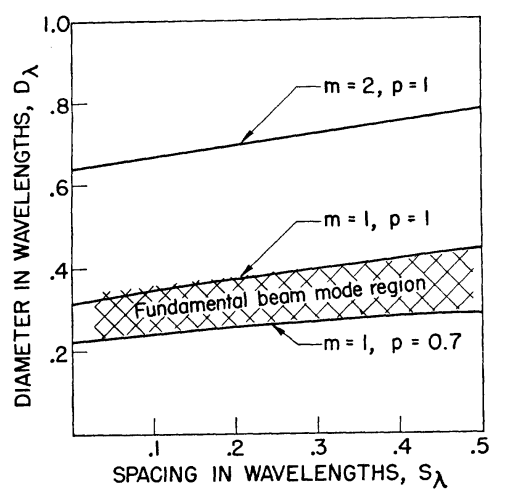
\includegraphics[width=0.4\textwidth]{diametro_espaciado.png}
	\caption{Diámetro vs espaciado}
	\label{fig:diam_vs_spacing}
\end{figure}

La factor de velocidad de fase debe estar entre $p=1$ y $p=0,7$ 


\newpage
\bibliographystyle{plain}
\bibliography{biblist}
\newpage

\printglossary[type=\acronymtype]

\newpage
\printglossary[type=main]

\end{document}